\subsection{Introducción:}

En este ejercicio nos encargaremos del manejo de las interrupciones del reloj, teclado y otra interrupcion de software 0x46. Se pide:

\begin{itemize}
\item [\textit{a)}] Completar las entradas necesarias en la IDT
\item [\textit{b)}] Escribir la rutina asociada a la interrupcion de reloj, de manera que por cada tick, se muestre la animacion de un cursor rotando
\item [\textit{c)}]  Escribir la rutina asociada a la interrupcion de teclado, para aquellas teclas a utilizar en el juego, para que se imprima la misma en la pantalla
\item [\textit{d)}] Escribir la rutina asociada a la interrupcion de software 0x46 para que modifique el valor de eax por 0x42
\end{itemize}



\subsection{Ítem a): Completar la \textit{IDT}}

Comenzamos agregando las interrupciones a la IDT. Utilizamos para el reloj y el teclado las posiciones 32 y 33 respectivamente, pues son las primeras disponibles no utilizadas por el procesador. Para la interrupcion por software, utilizamos la posicion 70, pues esta se llamara al llamar a int 0x46 $=$ 70. Las declaramos con privilegio 0, pues son de sistema y no se querria que algo externo al sistema los controle. \\
Para esto utilizamos la macro anteriormente explicada, con los siguientes parametros:

\begin{figure}[H]
\begin{center}
\minipage{0.25\textwidth}
  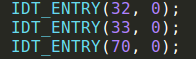
\includegraphics[width=\linewidth]{ejercicio5/idt.png}
\endminipage
\end{center}
\end{figure}

Ademas, las definimos en isr.h, para luego escribir su rutina.

\begin{figure}[H]
\begin{center}
\minipage{0.25\textwidth}
  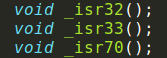
\includegraphics[width=\linewidth]{ejercicio5/isr.png}
\endminipage
\end{center}
\end{figure}

\subsection{Ítem b): Rutina del reloj}

El codigo es el siguiente:
\begin{figure}[H]
\begin{center}
\minipage{0.5\textwidth}
  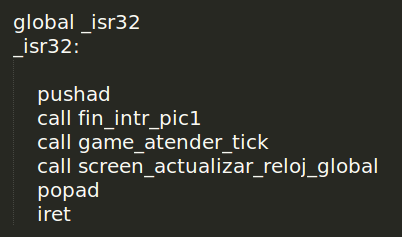
\includegraphics[width=\linewidth]{ejercicio5/rutinaReloj.png}
\endminipage
\end{center}
\end{figure}

Cada vez que se llame, la interrupcion hara lo siguiente. Pusheara todos los registros de proposito general (lo cual en realidad no es necesario, dado que la interrupcion no los modifica). Llamara a la funcion fin$\_$intr$\_$pic1 para decir al pic que la interrupcion fue atendida. Luego llamara a las funciones game$\_$atender$\_$tick y screen$\_$actualizar$\_$reloj$\_$global para mostrar la animacion por pantalla. Luego popeara los registros y volvera de la interrupcion con la instruccion iret


\subsection{Ítem c): Rutina del teclado}

El codigo es el siguiente:
\begin{figure}[H]
\begin{center}
\minipage{0.35\textwidth}
  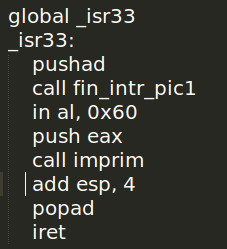
\includegraphics[width=\linewidth]{ejercicio5/rutinaTeclado.png}
\endminipage
\end{center}
\end{figure}

Igual que la interrupcion anterior, comienza pusheando todos los registros. En este caso, es necesario preservar eax, pues lo modificamos. Nuevamente llamamos a fin$\_$intr$\_$pic1. Luego utilizamos la operacion in, para mover al registro al el 
Leemos del teclado a traves del puerto 0x60 y obtenemos el scan code en eax. Pusheamos este valor y llamamos a la funcion imprim creada por nosotros. Esta funcion se encarga de traducir el scan code en una letra (en caso de que sea valido) y luego llama a la funcion print para mostrarlo por pantalla. Finalmente restauramos la pila, popeamos los registros y volvemos de la interrupcion

\subsection{Ítem d): Rutina 0x46}


El codigo es el siguiente:
\begin{figure}[H]
\begin{center}
\minipage{0.3\textwidth}
  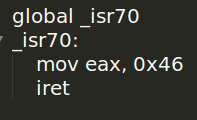
\includegraphics[width=\linewidth]{ejercicio5/rutina0x46.png}
\endminipage
\end{center}
\end{figure}

Lo unico que hace esta interrupcion es modificar el registro eax. Por lo tanto no es necesario salvar los registros. Esta interrupcion sera modificada mas adelante